%%%
%%% introduction.tex
%%%

%\subsection{Introduction}
\label{sec:dynamic_intro}
%%%
%%% Peering
%%%
Service providers in the core of the Internet connect to each other in
order to reach their respective customers.  Before agreeing to
``peer,'' two service providers sign a peering agreement that outlines
the terms of their relationship.  These contracts typically require
the Autonomous Systems (ASes) to connect in multiple geographic
locations~\cite{www-aol}; in Figure~\ref{fig:hotpotato}, ASes
$A$ and $B$ peer in four locations spread throughout their networks.
In addition to providing redundancy, the multiple connections are
meant to give an AS the flexibility to select a convenient egress
point for sending traffic to the other AS.  Under the common practice
of {\em hot-potato\/} (or {\em early-exit\/}) routing, a router
selects the ``closest'' egress point in terms of the intradomain path
costs, in order to reduce the network resources required to carry the
traffic.  For example, in Figure~\ref{fig:hotpotato}, router $b$ in AS
$B$ can direct traffic through peering point $3$ rather than sending
traffic a long distance across the network to one of the other egress
points.  Similarly, router $a$ in AS $A$'s network can direct traffic
through peering point $0$.  In some cases, a network operator may
override hot-potato routing
%(\eg, to select peering point $1$ rather than $0$)
to balance the traffic load.

%%%
%%% Consistent export
%%%
To give operators the flexibility to select from multiple egress
points, peering contracts typically require the peer to provide {\em
consistent\/} routes at all interconnection points~\cite{www-aol}.  That
is, an AS must make each destination reachable at every peering point
via ``equally good'' routes.  If a destination connected to router $a$
were reachable only through peering point $0$, traffic from $b$ would
have to travel over expensive long-haul links in AS $B$ and only a
short distance in AS $A$.  In this scenario, AS $A$ is violating its
peering agreement by {\em forcing\/} AS $B$ to do ``cold potato''
routing.  In addition,
% to making each destination reachable via all
%peering links, 
AS $A$ must not try to make one peering connection look less
attractive to $B$ than another (\eg, by making the AS path appear
longer), unless the two ASes have agreed in advance, since this would
force $B$ to consume more resources to send traffic.

\begin{figure}[h!]
\centerline{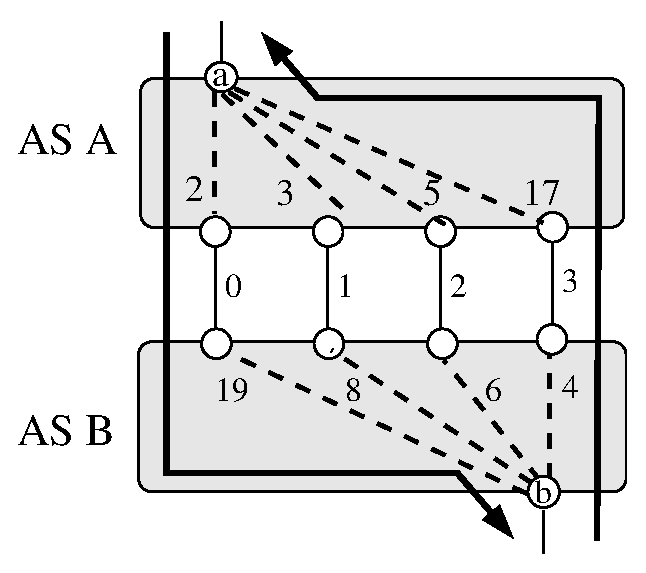
\epsfig{file=dynamic/figures/hotpotato.eps,width=0.4\textwidth}}
\caption[Hot-potato routing between ASes]{Hot-potato routing between
ASes with four peering points: 
  Dashed lines highlight the intradomain path costs} 
\label{fig:hotpotato}
\end{figure}


%%%
%%% What we do
%%%
In this section, we formulate the problem of checking the consistency of
routes advertised by a peer and present a technique for detecting
inconsistencies using routing and configuration data available in the
receiving AS.  The most closely related work is an empirical study of ``path
inflation'' by Spring {\em et al.}~\cite{Spring2003}, which analyzed
traceroute data to infer deviations 
from ``early exit'' routing without identifying the underlying
reason. 
In contrast, we determine whether an AS is {\em forced\/} to select a
different egress point due to inconsistent route advertisements from a
peer rather than {\em voluntarily\/} choosing a different egress point
to satisfy its own traffic engineering goals.

%%%
%%% BGP -- session per location, prefix everywhere, AS path length
%%%        (MED and origin type in footnote), distributed so hard
%%%
An AS receives route advertisements from a peer via Border Gateway
Protocol (BGP) sessions at the peering points.  
%BGP is a path-vector protocol that operates at the level of IP prefixes.  
A BGP-speaking router sends an advertisement to notify its neighbor of
a new route to the destination prefix and a withdrawal when the route
is no longer available.  An advertisement includes attributes, such as
the list of ASes in the path, that affect the selection of the best
route at each router.  To be consistent, multiple routes from the same
peer for the same prefix must agree in any aspects that affect the BGP
decision process---AS path length, origin type, and multiple exit
discriminator (MED)---as shown in bold in Table~\ref{tab:decision}.
Other steps in the decision process are controlled by the receiving
AS.  For example, a router can apply an import policy that assigns the
local-preference attribute to favor one route over another, and use
the intradomain path cost to select the route with the closest egress
point.  Although the operator can configure an import policy that
resets the origin type and MED attributes to default values, the
receiving AS is especially vulnerable to inconsistencies in the AS
path lengths of the routes advertised by its peers.

\begin{table}
\begin{small}
\begin{center}
\begin{tabular}{|l|} \hline
1. Highest local preference \\
{\bf 2. Lowest AS path length}\\
{\bf 3. Lowest origin type}   \\
{\bf 4. Lowest MED (with same next-hop AS)} \\
5. eBGP-learned over iBGP-learned \\
6. Lowest intradomain path cost to egress point \\
7. Lowest router ID of BGP speaker \\
\hline
\end{tabular}
\end{center}
\end{small}
\caption{BGP decision process with peer-assigned attributes in bold}
\label{tab:decision}
\end{table}

%%%
%%% Algorithm
%%%
Identifying inconsistencies should be as easy as comparing the BGP
routes learned from each peer for each prefix for differences in AS
path length, origin type, and MED, as discussed in
Section~\ref{sec:problem}.  Unfortunately, acquiring a feed of {\em
all\/} routes advertised by a neighboring domain is difficult in
practice\footnote{This would require either (1) extending today's
commercial routers to provide a feed of all eBGP-learned routes,
which, while definitely appealing, is not likely to happen quickly,
(2) deploying packet monitors on the many high-speed links between
peers to capture the BGP updates, which would be extremely
expensive, or (3) asking the peer AS to provide the eBGP data feed
from its own border routers, which runs the risk that the peer
intentionally sends {\em different\/} information to our detection
algorithm than it does to the operational routers.}.  Instead, we
consider how to detect inconsistent routes from data readily available
within the local AS---an internal BGP (iBGP) feed of the ``best''
route for each prefix from each border router and the import policies
configured on each of these routers.  However, identifying
inconsistencies from this data is challenging because our algorithm
only has access to the ``best'' route for each prefix, after the
routes have been manipulated by the import policies.  In
Section~\ref{sec:algo}, we determine how much these constraints limit
our ability to identify inconsistent route advertisements from peers
and present an algorithm that identifies inconsistencies that force
the AS to select a different egress router.


%%%
%%% The rest of the paper
%%%
Section~\ref{sec:results} presents the results of applying the
algorithms to the routes advertised by the peers of AT\&T's commercial
IP backbone.  We apply the first algorithm to eBGP feeds provided by
one large peer and then apply the second algorithm to iBGP feeds from
AT\&T's border routers.  Our analysis discovers many short-lived
routing inconsistencies that could be explained by transient routing
updates during the BGP convergence process, but we also find
inconsistencies that persist for longer periods of time, suggesting
either configuration mistakes or malicious behavior.  In
Section~\ref{sec:expl}, we present several examples that illustrate
how a peer might {\em inadvertently\/} advertise inconsistent routes
and suggest ways the sending AS could detect potential problems in advance.
Section~\ref{sec:concl} concludes the section with a discussion of ways
router vendors and network operators can make the BorderGuard problem
easier to solve in the future.
